

\documentclass[12pt,a4paper]{book}



			% Packages Files
%----------------------------------%

	% Page Setttings
\usepackage[top = 1in, bottom = 1in, left = 1in, right = 1in]{geometry}

\parindent=0cm % to prevent the spacing in new paragraph or new line

\usepackage{fancyhdr} % needded for header and footer 

%-----------------------------------------------------------------%

\usepackage{amsmath} % needed for referencing thequation
\usepackage{amsfonts} % for maths symbols
\usepackage{graphicx}
\usepackage[export]{adjustbox}
\usepackage{caption}
\usepackage{refstyle} % to reference a captioned figure


% To make hyperlinks

\usepackage[
	colorlinks=true
	,breaklinks
	]{hyperref} % needed for creating hyperlinks in the document, the option colorlinks=true gets rid of the awful boxes, breaklinks breaks lonkg links (list of figures),
	
\usepackage{xcolor}
\definecolor{c1}{rgb}{0,0,1} % blue
\definecolor{c2}{rgb}{0,0.3,0.9} % light blue
\definecolor{c3}{rgb}{0.3,0,0.9} % red blue
\hypersetup{
    linkcolor={c1}, % internal links
    citecolor={c2}, % citations
    urlcolor={c3} % external links/urls
}

	% For Code Writing
	
\usepackage{listings}

\usepackage{color}

\definecolor{mygreen}{rgb}{0 0.6 0}

\lstset{
% Set automatic Line breaking, in case we have long lines don't
% fit inside the frame or the page.
breaklines = true,
commentstyle = \color{mygreen},
breakatwhitespace = true,% don't show white space character
%numbers = left, % put line number in the code
keywordstyle=\color{blue}
title = \lstname
}

% ------------- For Writing Equations inisde a table and centering them ------------

\usepackage{array}

% Vertical Alignment inside the cells of the table
\newcolumntype{M}[1]{>{\centering\arraybackslash}m{#1}}

% Horizontal Alignment inside the cells of the table
\newcolumntype{P}[1]{>{\centering\arraybackslash}p{#1}}

% Wrting list inside a table

% \usepackage[shortlabels]{enumitem}
 
% \usepackage[shortlabels]{enumitem}

% -------- Multi Row Table------------
\usepackage{multirow}

% %---------- needed for long tables over pages-------
\usepackage{longtable} 


\usepackage{subfig}
% To adjust the page style
\usepackage{fancyhdr}


% needed for todos liste
\usepackage{todonotes} 


% ----------------- Tikz Package --------------

\usepackage{tikz}

\usetikzlibrary{shapes,shadows,arrows}

\usetikzlibrary{calc}






% Macros File

% Macros Example
\def\labelaxes{Remember to include some suitable labeling for the axes and the units used in measurements.}

% 2nd way for defnining macros: the new command
% 1st parameter: name of the new command
% 2nd paramter: how many inputs this command needs, in this case only 1
% 3rd parameter: what this new command named \tbi do

\newcommand{\tbi}[1]{\textbf{\textit{#1}}}

% Command for Picture without a label

\newcommand{\pic}[3]{\begin{figure}[h]
\centering
\includegraphics[width = 0.7\textwidth, frame]{#1}
\caption{#2}
\end{figure}}








\DeclareMathOperator*{\argmax}{argmax} % thin space, limits underneath in displays

\DeclareMathOperator*{\argmin}{argmin}

\title{System Programming in C}
\author{Ranim Tom}



\begin{document}

% downloaded template
%\input{content/title_page_1} 

%\maketitle
\tableofcontents


% to make the todo list appear as a table of content
\listoftodos

\pagestyle{fancy}
\fancyhf{} % Clear header and footer
\rhead{\rightmark}
\lhead{Chapter \thechapter}
\rfoot{Page \thepage}

\chapter*{Abstract}

The goal of this reader is to summarize my learning in system programming in \verb|C|.

\chapter{Introduction}

\section{System programming concepts}

\begin{itemize}

\item purpose for user mode: user application software must prevent to access the hardware directly, because it could damage the hardware.

Hence the kernel provide a layer between the user application and the hardware.

\item If a user program needs to access hardware,  it will be done via the kernel mode

    \begin{itemize}
        \item In this mode, we have a set of calls and programs to access the hardware

        \item Once the required information is fetched from the hardware,  it will be passed to user application
    \end{itemize}

\item What is  a kernel?

The kernel is the core of an OS, which handles resources.

It resides inside the memory, and it is the $\mathrm{1}^\mathrm{st}$ thing that comes at the start of a bootloader


\item Function of a kernel

    \begin{itemize}
    
    \item file management

    \item  memory management: making the memory available to different processes via the virtual memory management


    \item Interprocess communication: how different processes communicate with each other

    \item Threads (so multitasking system)
    \end{itemize}


\item Linux as layer view

\begin{itemize}
    \item Linux hide hardware from direct access by user application, because if so it can damage the hardware

    \item \todo{Linux layer} \textit{Linux layer: to insert a picture later}
\end{itemize}

\item When accessing hardware, the OS turns into kernel mode

    \begin{itemize}
        \item \todo{kernel mode} \textit{kernel mode: to see if this is called also privilege mode}
    \end{itemize}

\end{itemize}


\todo{kernel function} \textit{kernel functions and concept}

\begin{itemize}

\item \textit{to define and write later different new concept used, like what is a process, a  thread, concepts about Linux OS, $\cdots$}

\item \textit{Add references about system programming later}

\end{itemize}


\newpage
\section{System Call}


\subsection{Library}

Before diving into system call, let's fix the terminology first.

In a normal \verb|C| program, we need to include \tbi{header files} to use some function, such as \verb|stdio.h| to use \verb|printf()|.
This type of library is called \tbi{C standard library}.\\

\subsection{Getting into system call}

Now in system programming, we have some libraries which are designed to operate in a system call.\\

So what is a system call?\\

System calls (often shortened to \textit{syscalls}) are function invocations made from user space—your text editor, favorite game, and so on—into the kernel (the core internals of the system) in order to request some service or resource from the operating system (chapter 1 in \cite{book_Linux_System_Programming_Robert_Love}) 



\begin{itemize}

\item  The programs run in a kernel mode during system call execution

\item There are 2 ways to perform system call:

\begin{itemize}
    \item Or using directly the kernel like the function \verb|write()|
    
    \item Through a library function.

    Example is \verb|prinf()| which in turns call \verb|write()|

\end{itemize}

\end{itemize}

\newpage
\subsection{Internal mechanism for system call}

\begin{itemize}
    
\item The functional block diagram is shown in \autoref{fig:concept_system_programming:sys_call_diagram}.

\begin{figure}[h]
\centering
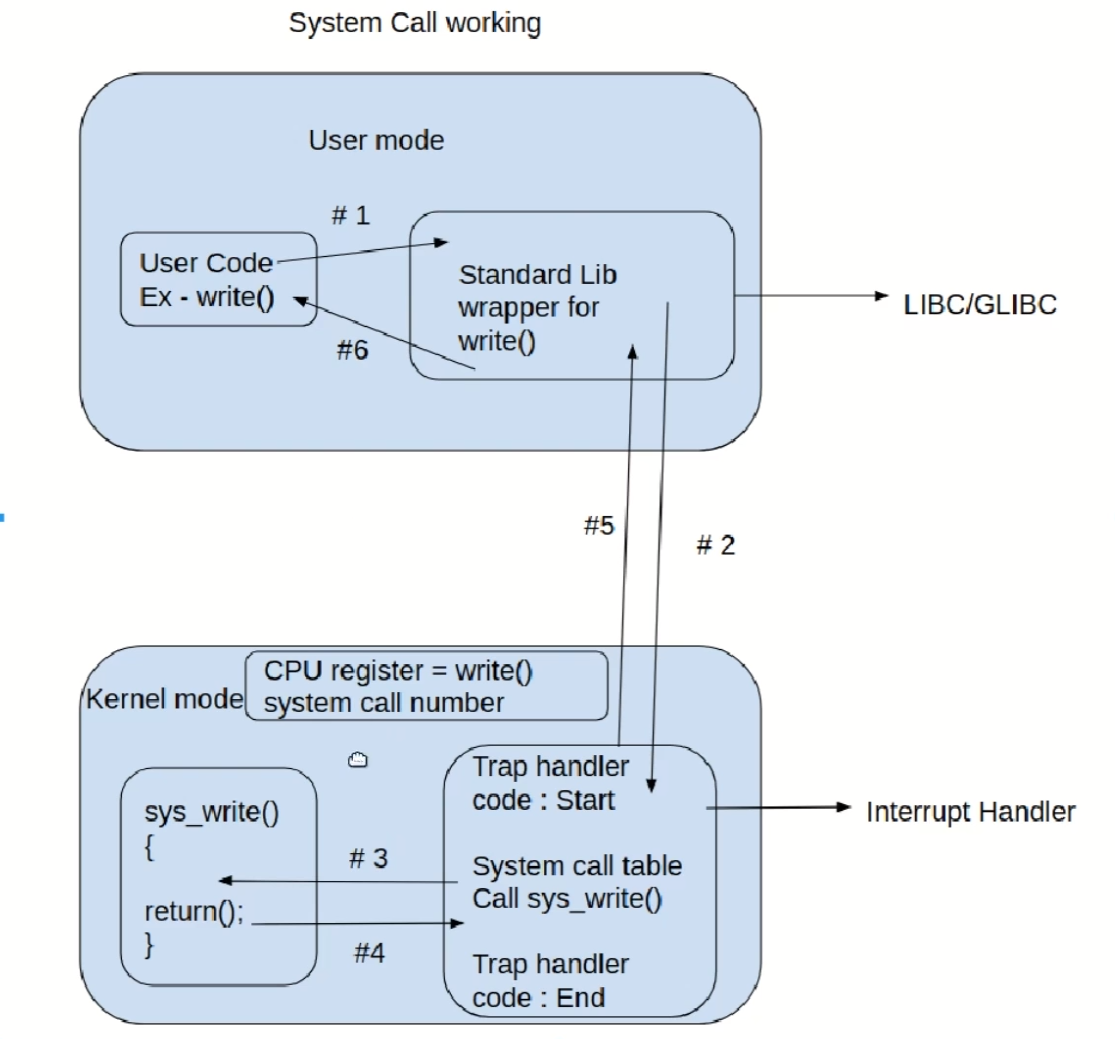
\includegraphics[width = 0.7\textwidth, frame]{Figures/concept_system_programming/sys_call_diagram}
\caption{Main Components}
\label{fig:concept_system_programming:sys_call_diagram}
\end{figure}


\item Every system call has a unique number associated with it 


\item When we use \verb|write()| function in our code, it will no directly invoke the definition (implementation), rather it will call a \tbi{wrapper}

\item This wrapper will raise an interrupt specific to hardware, and will compare the number associated to this function, in order to search to system call actual definition

\item Finally we will get to the actual function and get back the outputs

\item  Then we turn our way up to the user space again with the correct output.

\end{itemize}


\chapter{File I/O}

\section{Introduction}

Now we move for file manipulation in system programming.

Files are important in linux system programming, because everything is a treated as file in linux (chapter in 1 in \cite{book_Linux_System_Programming_Robert_Love}).\\


\underline{Under the hood info:}

\begin{itemize}
    \item Once we open a file, a metadata is attached to this open state is called file descriptor, known as \verb|ftd|, which is handled as \verb|int| \verb|C| type.
\end{itemize}


\section{File types}

There exist many file types in system programming, as shown in \autoref{fig:files:file_types}.

\begin{figure}[h]
\centering
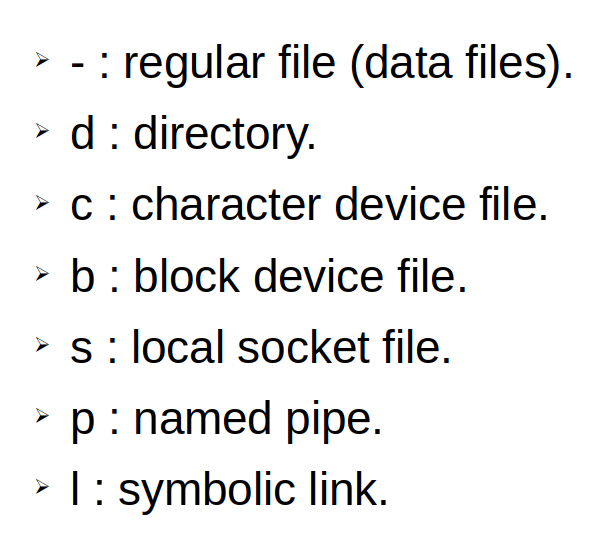
\includegraphics[width = 0.7\textwidth, frame]{Figures/files/file_types.png}
\caption{File types}
\label{fig:files:file_types}
\end{figure}



%====================================================
%====================================================
%====================================================

\chapter{Processes}

\section{References}

\begin{itemize}

\item chapter 5 in \cite{book_Linux_System_Programming_Robert_Love}

\item chapter 2 in \cite{book_modern_operating_system}

\end{itemize}

\section{Introduction}

In this section I will present multiple defintions in order to have a complete picture about processes.\\


\underline{$\mathrm{1}^\mathrm{st}$ definition:}\\

Processes are next to files, the $\mathrm{2}^\mathrm{nd}$ important abstraction unit in Unix (and OS in general) system.

In simple terms, we can define a process a program being executed such as \verb|C| program.

But a process is also much bigger than that: it contains kernel resources, virtualized memory, many threads,$\cdots$.\\

\underline{2nd definition of a processe:}\\

Imagine we have some program written in some high level language such as \verb|C| or \verb|java|. Computers doesn't understand high level languages, this why we have compilers that compile our code, and transfrome it into an binary executable.

However, this binary executable is not enough to run the program, it needs to be \tbi{loaded into the memory}, and allocate some resources. The OS is the brain which will do so.

Once the program start running, \textit{at this moment}, we can call it a process.\\

\subsection{Threads}


Now we move to the $\mathrm{2}^\mathrm{nd}$ concepts which is thread. Thread is the basic unit wihtin a process. A process can have from 1 thread to many threads.


\subparagraph{Programs, Process, Threads}

It should be noted that a program (for example a web browser) can have multiple process, and same between processes and threads.

\subsection{Visualizing processes}

\todo{Visualizing processes} \underline{\textit{Visualizing processes}:}

\begin{itemize}

\item \textit{To insert the commands in Linux with some iamges}

\end{itemize}



Some concepts:

\begin{itemize}

\item a process is an exected program (such as a build \verb|C| program)

\end{itemize}

\todo{Process Intro} \textit{Process Intro}

\begin{itemize}

\item \textit{To read later from books about processes, and the youtube videos I saw before}

\item \textit{To see the youtube playlist about processes}

\end{itemize}

\underline{youtube playlist}

\begin{itemize}

\item \url{https://www.youtube.com/watch?v=OrM7nZcxXZU&list=PLBlnK6fEyqRgKl0MbI6kbI5ffNt7BF8Fn}

    \begin{itemize}
        \item Neso Academy for operating systems

        \item Can serve as theory and complementary explanation for my books reading
    \end{itemize}

\item  \url{https://www.youtube.com/watch?v=cex9XrZCU14&list=PLfqABt5AS4FkW5mOn2Tn9ZZLLDwA3kZUY}

    \begin{itemize}
        \item nice playliste for examples in \verb|C|

        \item Contains alos a playlist for threads
    \end{itemize}

\end{itemize}

\section{Process ID}

\newpage
\section{Process states}

Now we have learned that a process is a program that is being executed (running).

While this program is running, its \textit{state is beign changed}, that is it passes from 1 state to another.

How we define the state of a program ? by the activity it is currently doing.\\

In \autoref{fig:processes:processes_states} we have the different state, and also how they are running.	


\begin{figure}[h]
\centering
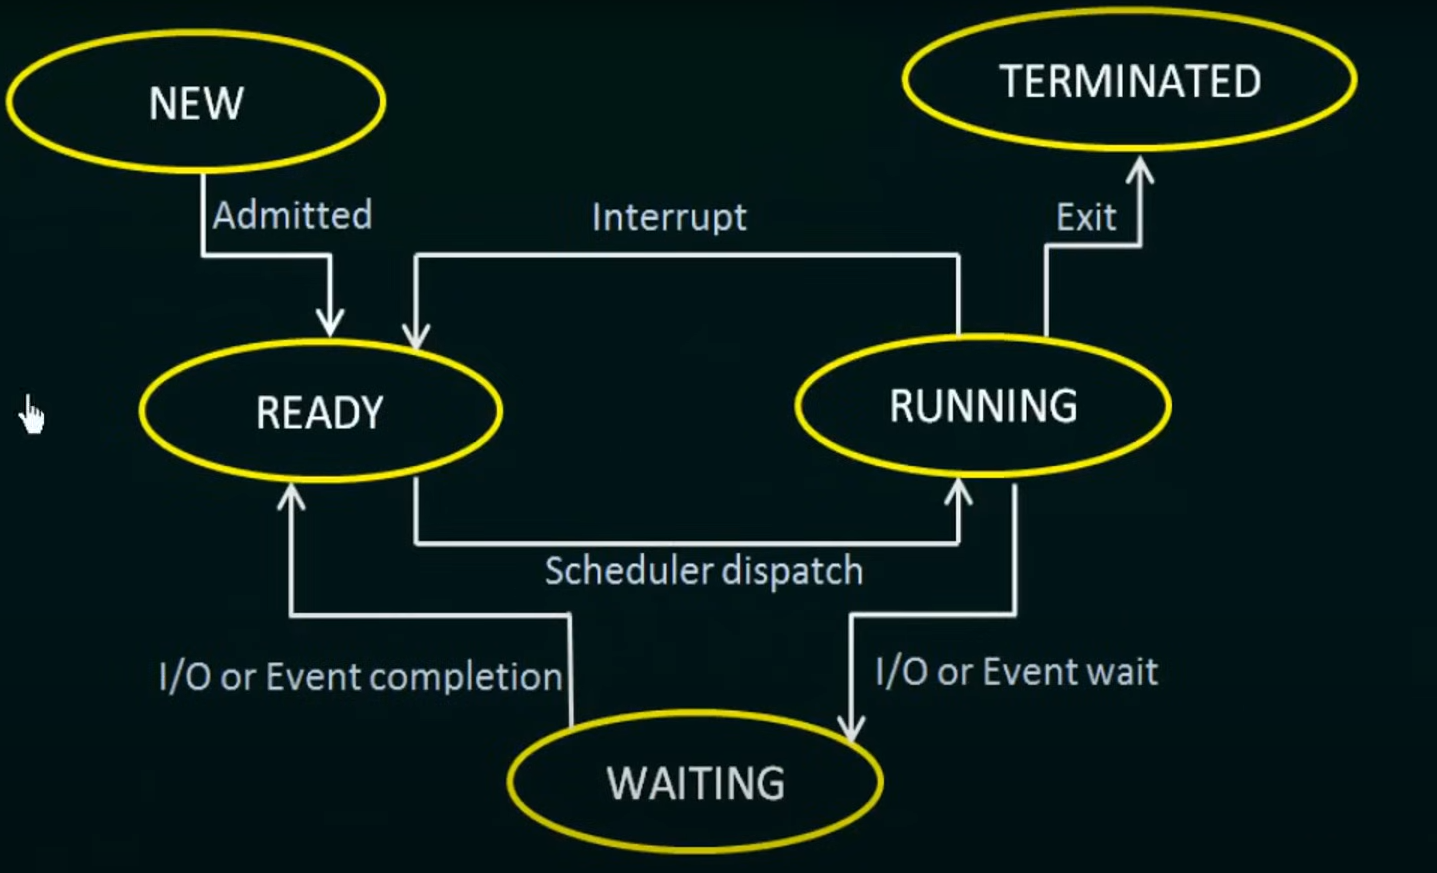
\includegraphics[width = 0.7\textwidth, frame]{Figures/processes/processes_states}
\caption{Different state of a process}
\label{fig:processes:processes_states}
\end{figure}

\begin{itemize}

\item New: is the creation of the processe.

\item Once the processe is being created, it enters into a ready staty to be assigned into a processor in order to run.

\item Now the process is assigned, it enter the running state, that is being executed and doing its job

\item After this running state, we have 3 cases:

	\begin{enumerate}
	
	\item terminate: this is the normal case, that is the process has not been interrupted in some way	
	
	\item the process get back to the ready state due to some interrupt signal , like some other process with higer priority need to be run.
	
	\item Finally, the current process maybe need some I/O or some signals. In that case, the process enter a waiting state in order to have these informations	
	
	\end{enumerate}



\end{itemize}

\newpage
\section{Process Control Block}

Each process is represented by the OS by a process control block (PCB). An example is shown in \autoref{fig:processes:pcb_example}.


\begin{figure}[h]
\centering
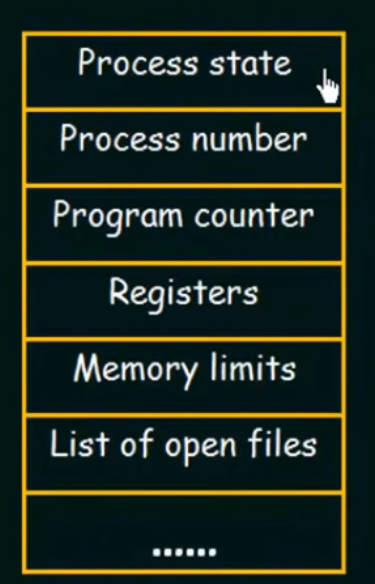
\includegraphics[width = 0.3\textwidth, frame]{Figures/processes/pcb_example}
\caption{Process control block example}
\label{fig:processes:pcb_example}
\end{figure}


\begin{itemize}


\item program counter: pointer which tells us the addresse of the next instruction (instruction of the code) that will be executed

\item Registers (CPU regsiters): tells us which registers are begin used by this process (like stack pointers, general purpose registers,$\cdots$).

\item Memory management information: section of the memory attached to this particular process

\item I/O status info: which I/O will be used by the procees


\end{itemize}


\newpage
\section{Process creation}

\underline{Important points of the video:} The following points are about the \verb|fork()| system call used to create processes in linux


\begin{itemize}

\item once \verb|fork()| is used to create the process, the child process will have the same resources as the parent process.

\item The special thing about \verb|fork()| is it returns value in 2 places:

    \begin{itemize}
        \item In the parent process, the process ID \verb|pid_t|

        \item In the child process, it returns -1 or error
        
    \end{itemize}

\item The child process execute the same program as the parent process

\item Each process can now modify their variables without affecting the other, and store in its correspondent memory segment (heap, stack,$\cdots$) 

\end{itemize}


In \autoref{fig:processes:fork_before_after}, we have the state of before and after. 

In other words, once we use the \verb|fork()| in some \verb|C| source file, starting from this line we have 2 branches (2 codes), each with a separate memory

\begin{figure}[h]
\centering
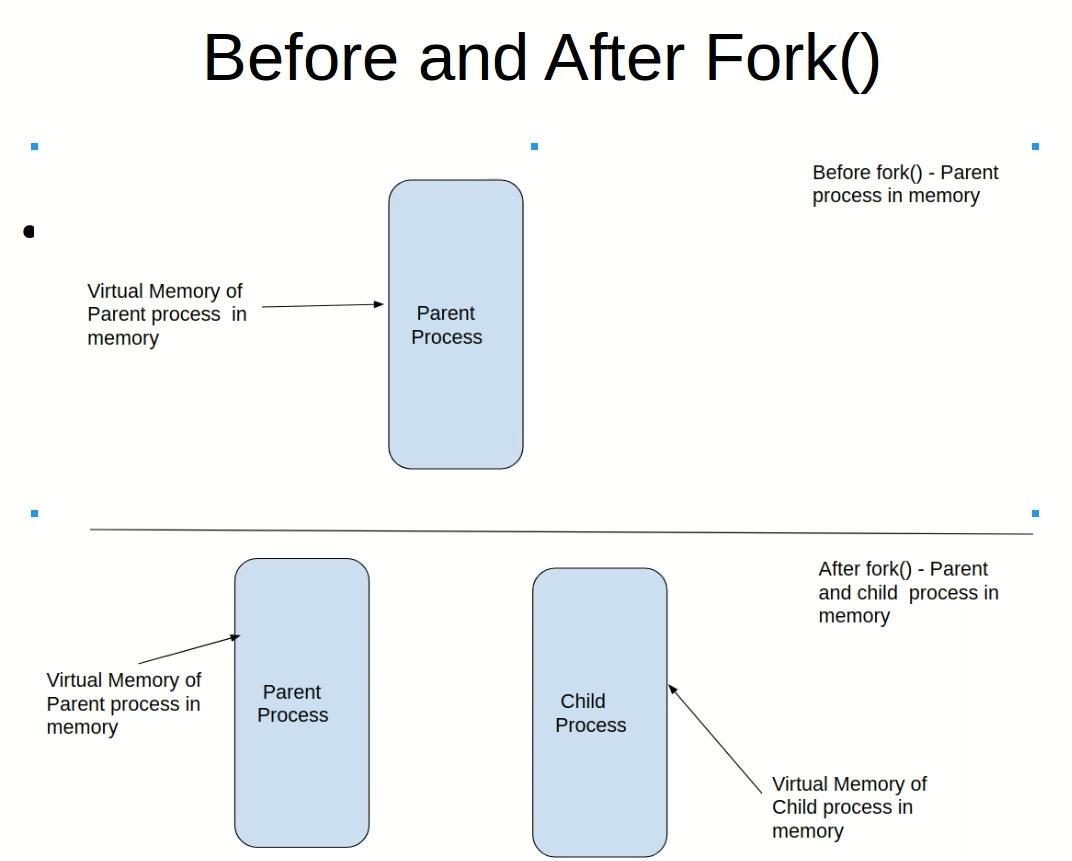
\includegraphics[width = 0.7\textwidth, frame]{Figures/processes/fork_before_after}
\caption{fork system call: before and after}
\label{fig:processes:fork_before_after}
\end{figure}

\subsection{Copy on- write}

We can see that in \autoref{fig:processes:fork_before_after} after \verb|fork()| is being called, that we have 2 memory section: once for each process. So we can say that the OS make a copy of the memory. This was the old style employed by Unix system.

Now in modern Unix system such as Linux, copy is note made  directly (to avoid unnecessary copy), and the 2 processes share the same memory. It is only when one of the processes need to alter or change some resources, copy will be made.

In other words, if one of the processes (parent or chlid) require some \tbi{modification of the data}, only then a separate memory will be duplicated.

Hence the name copy on write.\\

For further information about the mechanism, see chapter 5 in \cite{book_Linux_System_Programming_Robert_Love}.



\newpage
\section{Waiting a process}


\underline{Video 38 of the course}. I reached 29.37.\\


\todo{wating process motivation} \underline{\textit{wating process motivation}:}

\begin{itemize}

\item \textit{To write a better motivation for this section after reading from the references \cite{book_Linux_System_Programming_Robert_Love}, \cite{book_opearting_system_concepts}}

\end{itemize} 

\underline{Explanation:}

\begin{itemize}

\item \textit{To repharase it later}

\item usually when we have 2 processes (a parent and a child), the parent need to wait for the child in order to terminate, and not the other way around

	\begin{itemize}
	\item In other words, the child wait for the parent
	
	\item In that case, the child will be assigned some parent process
	
	\item This can cause a zombie process and we can have a memory leak 
	\end{itemize}

\item  Sometimes a process need to wait for the child process in order to terminate

\item  Each process which terminate has an exit status

\item terminating a process is done via the \verb|void exit(int status)|

    \begin{itemize}
        \item The important thing about this function is that it does not return anything to see if the a certain process is finished or not

        \item  We need to see the \verb|status| variable to know if the status has finished or not
    \end{itemize}

\end{itemize}

\todo{Video} \textit{Video course: video 38, at 20:17}.

\subsection{Functions}

\begin{itemize}

\item We have 2 functions to wait a process

\item Header: \verb|#include <sys/wait.h>|

\item \verb|int wait(int* status)| and 

\end{itemize}


\newpage
\section{Abnormal Processes}

\todo{Naming} \underline{\textit{Naming}:} 


\begin{itemize}

\item \textit{To see if I need to rename this section later.}

\end{itemize}

In this section we will see 3 special processes: orphane, zombine and sleeping process.

\begin{itemize}

\item If we have a parent and child process, and the parent process finish before the child (like it has exit), the child process will become an orphane process.

\end{itemize}


\subsection{Zombie process}

This section is from chapter 1 in  \cite{book_Linux_System_Programming_Robert_Love}.

\begin{itemize}

\item When a process terminates, it is not immediately removed from the system. 

\item Instead,the kernel keeps parts of the process resident in memory to allow the process’s parent to inquire about its status upon terminating. 


\item This inquiry is known as waiting on the terminated process. Once the parent process has waited on its terminated child, the
child is fully destroyed. 



\item A process that has terminated, but has not yet been waited upon, is called a zombie process.

\todo{zombie process} \underline{\textit{zombie process}} :
	
	\begin{itemize}
	\item \textit{To understand this sentence even more.}
	\end{itemize}

\end{itemize}


\todo{Zombie process concept} \underline{\textit{Zombie process concept}:} 

\begin{itemize}

\item \textit{To understand later the concept of zombie}

\item \textit{From what I understand from the video, if a child process exit before the parent process and its entry table remains, the child process is knonw as a zombie process}

\item \textit{Using} \verb|wait()| or \verb|waitpid()| \textit{in the parent process resolve the issue}

	\begin{itemize}
	\item \textit{To dig more why this is the solution}
	\end{itemize}

\end{itemize}

\newpage
\section{Memory Layout}
Now we discuss memory layout for the process.

Memory a of process is composed of different \tbi{segments} as enumerated below

\begin{enumerate}

\item Text: code reside here

    \begin{itemize}
        \item that is the code of the program is being executed

        \item this segment is a \textit{read only} $\leftrightarrow$ can't be altered by any pointer
    \end{itemize}

\item Data: data variables during compile time

    \begin{itemize}
        \item It is composed between uninitialized and initialized data 
    \end{itemize}

\item  stack: for local variables and functions

    \begin{itemize}
        \item the composition inside the stack is called \textit{frame}

        \item each frame contains 1 functions and its related variables
    \end{itemize}

\item heap: dynamic variables

\end{enumerate}

\subsection{Code Example}

\todo{Code Example} \underline{\textit{Code Example:}}

\begin{itemize}

\item \textit{To do later some examples using some example programs}

\item \textit{To see video number 26 from the course, and examples from the books also}

\end{itemize}


\newpage
\section{Excec Family}

Till now we have see the \verb|fork()| funciton, which duplicate a program, \tbi{but the heap and the stack remains the same}.\\

Another form of creating process is through the \verb|exec| family fo calls. The difference here is:

	\begin{itemize}
	\item In this type of function, the program will load and execute some new process, and hence it will \tbi{replace the previous contents of the address space, and begin execution the new program} (see chapter 5 in \cite{book_Linux_System_Programming_Robert_Love}) 
	\end{itemize}


An example is shown in \autoref{fig:processes:excel_family_example}.

\begin{figure}[h]
\centering
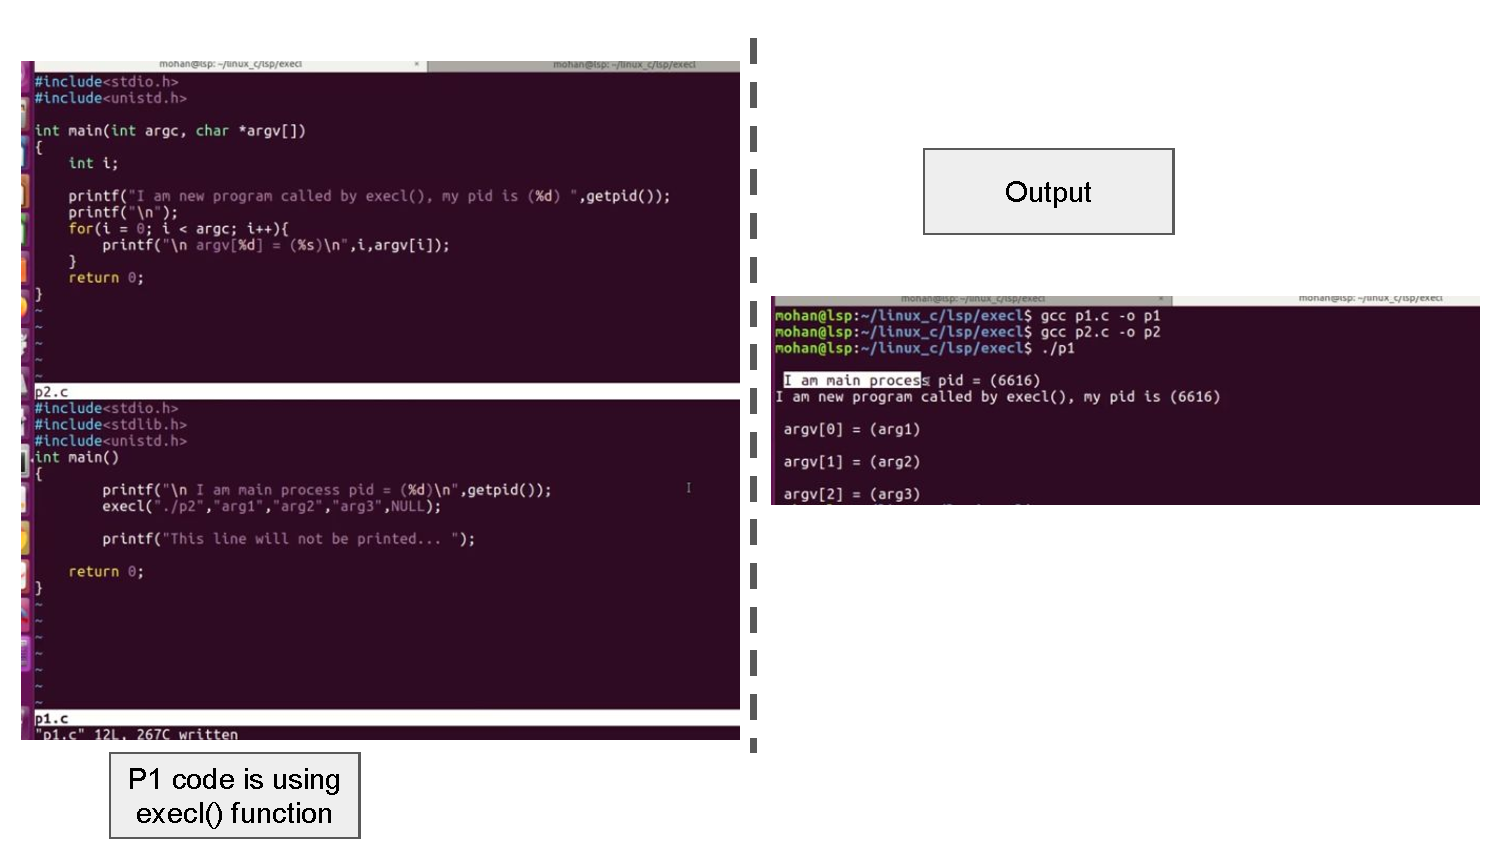
\includegraphics[width = 0.9\textwidth, frame]{Figures/processes/excel_family_example}
\caption{Excel() example}
\label{fig:processes:excel_family_example}
\end{figure}

	\begin{itemize}
	
	\item \verb|p1| is calling \verb|p2| using \verb|excel()|
	
	\item The arguments to \verb|excel()| are the binary (compiled 		code)
	
	\item Note that is because we have a replacement of memory, the \verb|printf()| for \verb|p1.c| is never executed
	
	\item Even we are running \verb|p2.c| from \verb|p1.c|, but we have the same process id in both
	
	\end{itemize}


\newpage
\section{Notes and summary}

\begin{itemize}

\item About the memory layout: a nice example about text segment and how it is read only, the code \verb|char* buff = "welcome"|.

    \begin{itemize}
        \item \verb|welcome| variable here is store in the text segment, so we can't change it

        \item If we try to do \verb|buff[0] = '\n'|, it will result in a segmentation fault
    \end{itemize}


\end{itemize}


\newpage
\section{TODO for Processes}

Thi section contains general idea for some points to do later for processes.

\begin{itemize}

\item Write a better introduction later for the begnning of this chapter

\item There is the concept of using \verb|fork()| and \verb|excel()| together in the same code

	\begin{itemize}
	\item This is the in the video 44 of the course
	
	\item But need to search better in the books for some practical apsect also, and not only theory
	\end{itemize}

\item To see also the ide of files handling in a \verb|fork()| call

	\begin{itemize}
	\item What happen to these resources before and after the \verb|fork()|
	
	\item For this I need to review the low level things about file handling (file as a byte, offsetting a file, $\cdots$)
	\end{itemize}

\end{itemize}



%=================================================
%=================================================
%=================================================

\chapter{Signals}

\section{Intro}

\underline{Section from course:} number 11

\begin{itemize}

\item Signals are interrups that provide mechanism to deal with some unexpected events

\item The signals comes from the kernel side

\item Every signal has a signal handler

	\begin{itemize}
	\item The signal handler is a juste function 
	\end{itemize}

\end{itemize}


Also some points from my reading in \cite{book_opearting_system_concepts} (chapter 4, section 6.2):

\begin{itemize}

\item Signals are ways to notify the process for some particular events

\item 2 types of signals:

	\begin{enumerate}
	\item synchronously: that is generated within the same process.
	
	Example can be a program that have done a division by 0, or accessing some illegal memory side
	
	\item asynchronously: the signal comes from outside the process, such pressing \verb|Ctrl C| to terminate a program (force it to terminate)

	\end{enumerate}


\item Once the signal is generated (either synchronous or asynchronous), \tbi{it must be handled by a handler}.

2 possible way to handle the signal:

	\begin{itemize}
	\item A default signal handler
	
	\item A user signal handler
	\end{itemize}


\item \underline{Default signal handler:} this is handled by the kernel, and we have 2 possibilities:

	\begin{itemize}
	\item can be ignored
	
	\item catch and handle the signal $\leftrightarrow$ 
	\end{itemize}

\item If a signal doesn't have a handler, it has a \tbi{default action to be taken}

\end{itemize}

\newpage
\section{Examples}

See example in \verb|signal| project in \verb|System Programming| workspace.\\

\todo{Alarm signal} \underline{\textit{Alarm signal}:}

\begin{itemize}

\item \textit{To redo the alram signla example because I didn't understand very clearly how the flow of the code is}

\end{itemize}


%=================================================
%=================================================
%=================================================

\chapter{Virtual Memory}


\section{The big picture}

The virtual memory concept allow the process to access more address space then the actual physical RAM.

\textit{Concept to be reviewed later:}

\begin{itemize}

\item \textit{Concept of an address space}

\item \textit{It's relation to the processes}  


\end{itemize}


\todo{Memory Management} \underline{\textit{Memory Management}:} \textit{I will redo this chapter later after the process chapter, and when the book arrive.} 


%===========================
%===========================
%===========================

\chapter{Threads}

\section{Introduction}

\todo{intro to thread} \textit{intro to thread}

\begin{itemize}

\item \textit{To write later the intro about the thread}


\item \textit{Difference between thread and processes}

\item \textit{Read from books}


\end{itemize}


\underline{Some points from the video lectures:}

\begin{itemize}

\item Different threads share the virtual memory with the process that created them

	\begin{itemize}
	\item Unlike processes, which can't share memory among 	each other
	\end{itemize}

\item In Linux, the most famous thread interface is \verb|POSIX|: abbreviation for portable operating system interfance

\item The advantage of having many threads is to have many threads is to divid a task into smaller one, and each handle by a thread.

\end{itemize}


\section{Race Condition}

In a high level, race conditions happen when a 2 threads try to access the same variable, and one of them has not finished yet.

\todo{Race Conditions points} \underline{\textit{Race Conditions points}:} 


\begin{itemize}

\item \textit{To revisit later the video number 3 in CodeVolt playlist}

\item \textit{To see what later to other points we can add from other videos or resources}

\end{itemize}

\subsection{Race Condition Question}

\todo{Race Condition Questions} \underline{\textit{Race Condition Questions}:} 

\begin{itemize}

\item Are threads happening in a parallel execution always, or they wait each other (overlapping manner) ?

\end{itemize}


\subsection{Mutex}

Mutex is a way to prevent race condition.

As a definition, a mutex is a lock about a section of code. \\

\underline{Some important points (taken from the CodVault playlist):}

\begin{itemize}

\item The idea is if we have 2 threads, by implementing the lock, there is no way we have a thread is reading, and the other thread will be executing

	\begin{itemize}
	\item In other words, the $\mathrm{1}^\mathrm{st}$ thread will finish its work
	\end{itemize}

\end{itemize}



\section{General Points}

\begin{itemize}

\item When we have 1 threads created, the thread and the main process share same process ID via the \verb|getpid()|.


\item When passing arguments to threads 

	\begin{itemize}
	
	\item this means we are passing input to the routine 		function
	
	\item This is done via \verb|pthread_create()|
	
	\item Don't forget that we need to cast the \verb|void*| pointer to the right type we are passing
		
	
	\end{itemize}

\item Whenever we create a thread, we need to wait this thread to be finish its work

	\begin{itemize}
	\item This is done via \verb|pthread_join()|
	
	\item The same is true if we have multiple threads.
	\end{itemize}

\item If we need to \tbi{return some result} (so \textit{an output}) from the thread

	\begin{itemize}

	\item We do it via \verb|pthread_join()|, using its $\mathrm{2}^\mathrm{nd}$ argument

	\end{itemize}

\end{itemize}


%========================================
%========================================
%========================================

\chapter{Libraries in C/C++}

\section{Introduction}

This chapter deal with external libraries in C/C++.


The libraries can be linked and loaded also via 2 options:

\begin{enumerate}

\item Static library and loaded statically

\item Dynamic library (or shared object in Linux \verb|.so|), which lnkied dynmaically.

\end{enumerate}


It is important to note that libraries are \tbi{precompiled files}, and we want to use them in our applications. The purpose of this precompilation is to save time and don't compile them each time we modify our code.

In other words, this means we compile only our source code, and the libraries remains intact.

\section{Some Tools}

\begin{itemize}

\item \verb|ldd some_output| command used to print out all the shared object dependcy related to our executable \verb|C| code, named \verb|some_output|.


\item An example is shown in \autoref{fig:Libraries:ldd_command_example}, where I genrate some executable named \verb|final_app|

\end{itemize}

\begin{figure}[h]
\centering
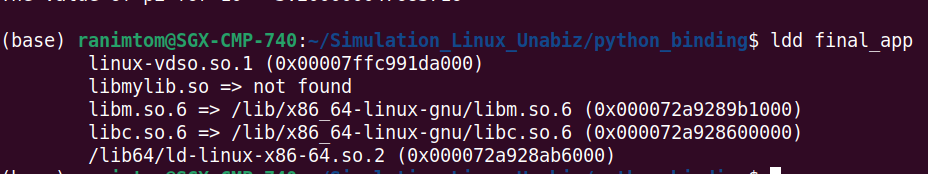
\includegraphics[width = 0.7\textwidth, frame]{Figures/Libraries/ldd_command_example}
\caption{ldd command example}
\label{fig:Libraries:ldd_command_example}
\end{figure}

\section{Static Libraries}

\begin{itemize}

\item Static libraries are binary files that are compiled using a compiler like \verb|gcc|

\item They result in a files with \verb|.o| extensions, which stands for object files

\item The important point about these libraries that they are \tbi{architecture dependent}, so if they run on my machine (Linux), doens't mean necessarly that they run on other machine

\item The final executable program will be big in size

	\begin{itemize}
	\item We can use the command \verb|ls -lh| to display the size of each fine in Kbytes
	\end{itemize}


\end{itemize}

\subsection{Creating a static library}

\begin{itemize}

\item Suppose we have 2 object files that we compile using \verb|gcc|. They are \verb|mymath.o| and \verb|mymath2.o|

\item To create the library, we need to bundle these 2 \verb|.o| files. We use \verb|ar| tool for this purpose.

\item The command will be:

\verb|ar rcs mymath.a mymath.o mymath2.o|, where:

	\begin{itemize}
	\item \verb|mymath.a| is the name of the librari, with \verb|.a| extension
	
	\item \verb|rcs| is for 
	\end{itemize}


\end{itemize}

\subsection{Pros and Cons}

\begin{itemize}
\item Static libraries are easy to deal with, since everything is bundled together, this simplifes distribution to other

\item but the size on disk and and at run time is big

\item Also the static libraries are not cross compiled $\leftrightarrow$ this means they can be shared by 1 program only

\end{itemize}


\section{Shared Library}

\begin{itemize}

\item shared library (or dynamic library) are another type, with \verb|.so| extension for Linux (and \verb|.dll| for window)

\end{itemize}

\subsection{Creating a shared library}

\begin{itemize}

\item \verb|gcc -fPIC -shared .src/mymath.c -o libmymath.so|

	\begin{itemize}
	\item This command instruct \verb|gcc| to create a shared library (hence the flag \verb|-shared|) named \verb|libmymath.so|
	
	\item \verb|lib| prefix is necessary for any name we choose, because the when compiling our code (see \ref{libraries_C:compiling_code_shared_lib}), the linker assume always the library name starts with \verb|lib|.
	
	\item Recall that \verb|-o| stands for output
	\end{itemize}

\end{itemize}


\subsection{Compiling C code with a shared library}
\label{libraries_C:compiling_code_shared_lib}

\begin{itemize}

\item Now once we create the shared library, we need to compile our \verb|C| code with this shared library

\item As any library, we need to link \verb|.so|  to our code using the linker (so using \verb|-l| flag)

\item Now this step is a little tricky

	\begin{itemize}

	\item Although our created shared library name is \verb|libmymath.so|, in the command we use only \verb|mymath|, where we omit both \verb|lib| (prefix) and the \verb|.so| extension
	
	\item The linker epxect these prefixes/postfixes so no need to add them in the command

	\end{itemize}


\item The command is:

\verb|gcc ./src/*.c -o prog -lmymath L./|

	\begin{itemize}
	\item \verb|.L/| is to indicate the the libraries are in the current directories
	\end{itemize}


\end{itemize}

\subsection{Running the program}

We use the following command using the environment variable:

\begin{itemize}

\item \verb|LD_LIBRARY_PATH="./" ./final_app|

\end{itemize}


%**************** References ****************

\bibliographystyle{IEEEtran}

\bibliography{Literature/Books_System_programming}



\end{document}
